% This example is meant to be compiled with lualatex or xelatex
% The theme itself also supports pdflatex
\PassOptionsToPackage{unicode}{hyperref}
\documentclass[aspectratio=1610, xcolor=dvipsnames, 9pt]{beamer}

% Load packages you need here
\usepackage{polyglossia}
\setmainlanguage{german}

\usepackage{csquotes}
\usepackage{smartdiagram}

\usepackage{amsmath}
\usepackage{amssymb}
\usepackage{mathtools}

\usepackage{hyperref}
\usepackage{bookmark}
\usepackage{tikz}
\usepackage{graphicx}
\usetikzlibrary{shapes.geometric, arrows, positioning, shapes.geometric, calc}

\tikzstyle{process} = [rectangle, rounded corners, minimum width=3cm, minimum height=1cm, text centered, draw=black, fill=orange!50]
\tikzstyle{arrow} = [thick,->,>=stealth]

% load the theme after all packages

\usetheme[
  showtotalframes, % show total number of frames in the footline
]{fhswf}

% Put settings here, like
\unimathsetup{
  math-style=ISO,
  bold-style=ISO,
  nabla=upright,
  partial=upright,
  mathrm=sym,
}

\title{Advanced Natural Language Processing/ Large Language Models}
\author[F.~Neubürger]{ \textbf{Felix Neubürger}}
\institute[I \& W]{Fachhochschule Südwestfalen, Ingenieurs- \& Wirtschaftswissenschaften}
\date{2025}
\titlegraphic{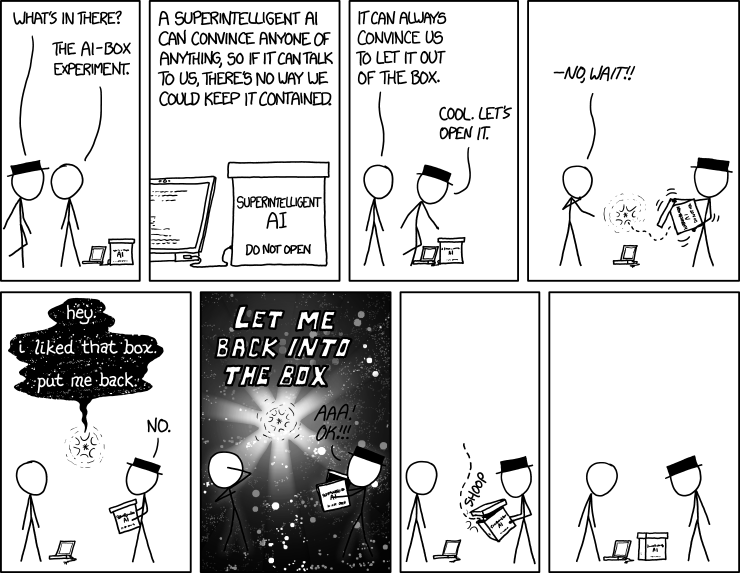
\includegraphics[width=0.2\textwidth]{images/ai_box_experiment.png}}


\begin{document}

\maketitle

\begin{frame}{Inhalte der Vorlesung}
  \begin{columns}
    \begin{column}{1\textwidth}
      \begin{itemize}
        \item Wie funktioniert Natural Language Processing\newline
        \item Sprachdarstellung zum Rechnen \newline
        \item Attentionmechanismus \newline
        \item Transformerarchitektur  \newline
        \item von BERT zu DeepSeek-v3 \newline 
        \item Wie es weitergehen kann \newline
        \item Nutzungsmöglichkeiten: RAG, Agentensysteme \newline
        \item AI Safety und Ethik \newline
        \item LLM Standardwerke 
      \end{itemize}
    \end{column}
    \begin{column}{0\textwidth}
% \begin{figure}
% \centering
%             \includegraphics[width=0.9\textwidth]{images/intro/intro.pdf}
% \end{figure}
    \end{column}
  \end{columns}
\end{frame}

\begin{frame}{Ziele der Vorlesung - Welche Fragen sollen beantwortet werden?}
  \begin{columns}
    \begin{column}{0.69\textwidth}
      \begin{itemize}
        \item Was sind die Grundlagen von Natural Language Processing (NLP)? \newline
        \item Wie funktionieren Attention-Mechanismen und warum sind sie wichtig? \newline
        \item Was ist die Transformer-Architektur und wie unterscheidet sie sich von anderen Ansätzen? \newline
        \item Wie werden Sprachmodelle wie BERT und GPT trainiert und genutzt? \newline
        \item Welche Herausforderungen und ethischen Fragen gibt es bei der Nutzung von LLMs? \newline
        \item Welche praktischen Anwendungen und Zukunftsperspektiven gibt es für LLMs? \newline
      \end{itemize}
    \end{column}
    \begin{column}{0.3\textwidth}
 \begin{figure}
 \centering
             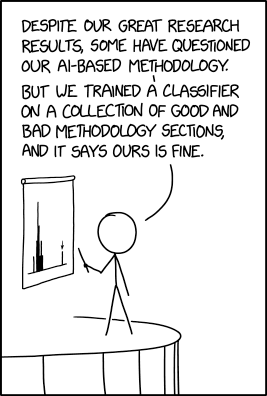
\includegraphics[width=0.9\textwidth]{images/ai_methodology.png}
             [\url{https://xkcd.com/2451/}]
 \end{figure}
    \end{column}
  \end{columns}
\end{frame}

\begin{frame}{Format der Vorlesung - Wie sollen diese Fragen beantwortet werden?}
  \begin{columns}
    \begin{column}{0.69\textwidth}
      \begin{itemize}
        \item Theroretischer Teil mit Folien \newline
        \item Praktischer Teil in Gruppen an einem Projekt  \newline
        \item Gruppengröße 2 oder 3 Personen \newline
        \item Einzelarbeit möglich wenn eigenes Thema vorhanden \newline
        \item Abgabe der Ausarbeitung einen Tag vor der Veranstaltung in der Blockwoche \newline
        \item Vorstellung der Projektergebnisse in der Blockwoche \newline
        \item Gewichtung der Bewertung Projektausarbeitung (50\%) und Vortrag (50\%)
        \end{itemize}
    \end{column}
    \begin{column}{0.3\textwidth}
 \begin{figure}
 \centering
             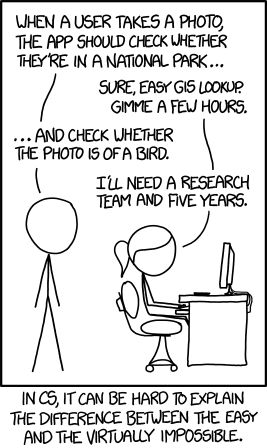
\includegraphics[width=0.7\textwidth]{images/tasks.png} \newline
             [\url{https://xkcd.com/1425/}]
 \end{figure}
    \end{column}
  \end{columns}
\end{frame}

% Abschnitt 1: Einführung in Natural Language Processing
\section{Wie funktioniert Natural Language Processing}

\begin{frame}{Wie funktioniert Natural Language Processing}
  \begin{itemize}
    \item Definition und Ziele des NLP \\
    \item Herausforderungen bei der maschinellen Sprachverarbeitung \\
    \item Anwendungen von NLP in der Praxis
  \end{itemize}
\end{frame}

\begin{frame}{Definition und Ziele des NLP}
  \begin{itemize}
    \item NLP steht für Natural Language Processing, die Verarbeitung natürlicher Sprache durch Computer.
    \item Ziel: Maschinen ermöglichen, menschliche Sprache zu verstehen, zu interpretieren und zu generieren.
    \item Anwendungen: Übersetzungen, Chatbots, Textanalyse, Sprachassistenten.
  \end{itemize}
\end{frame}

\begin{frame}{Herausforderungen bei der maschinellen Sprachverarbeitung}
  \begin{itemize}
    \item Ambiguität: Mehrdeutigkeit in der Sprache.
    \item Kontextabhängigkeit: Bedeutung hängt vom Kontext ab.
    \item Umgang mit Synonymen und Homonymen.
    \item Verarbeitung großer Datenmengen und Rechenaufwand.
  \end{itemize}
\end{frame}

\begin{frame}{Anwendungen von NLP in der Praxis}
  \begin{itemize}
    \item Sentiment-Analyse: Erkennung von Meinungen in Texten.
    \item Maschinelle Übersetzung: Automatische Übersetzung zwischen Sprachen.
    \item Sprachgesteuerte Assistenten: Siri, Alexa, Google Assistant.
    \item Textzusammenfassung: Automatische Erstellung von Textzusammenfassungen.
  \end{itemize}
\end{frame}

\begin{frame}{Text Preprocessing Pipeline}
  \begin{tikzpicture}[scale=0.8, transform shape]
    % Main arrow
    % Large arrow
    \fill[blue!50] (-1.5,-1.5) -- (10.5,-1.5) -- (10.5,-2) -- (17.5,0) -- (10.5,2) -- (10.5,1.5) -- (-1.5,1.5) -- cycle;

    % Process boxes
    \node (step1) [process, xshift=0cm] {Data Cleaning};
    \node (step2) [process, right of=step1, xshift=2.5cm] {Tokenization};
    \node (step3) [process, right of=step2, xshift=2.5cm] {Normalization};
    \node (step4) [process, right of=step3, xshift=2.5cm] {Stopword Removal};
    \node (step5) [process, right of=step4, xshift=2.5cm] {Vectorization};

    % Arrows connecting steps
    \draw[arrow] (step1.east) -- (step2.west);
    \draw[arrow] (step2.east) -- (step3.west);
    \draw[arrow] (step3.east) -- (step4.west);
    \draw[arrow] (step4.east) -- (step5.west);
  \end{tikzpicture}
\end{frame}

\begin{frame}{Data Cleaning}
  \begin{itemize}
    \item \textbf{Definition:} Entfernen oder Korrigieren von fehlerhaften, unvollständigen oder irrelevanten Daten.
    \item \textbf{Schritte:}
      \begin{itemize}
        \item Entfernen von Sonderzeichen, HTML-Tags und Emojis.
        \item Korrektur von Rechtschreibfehlern.
        \item Vereinheitlichung von Groß- und Kleinschreibung.
      \end{itemize}
    \item \textbf{Ziel:} Verbesserung der Datenqualität für nachfolgende Verarbeitungsschritte.
  \end{itemize}
\end{frame}

\begin{frame}{Tokenization}
  \begin{itemize}
    \item \textbf{Definition:} Zerlegung von Text in kleinere Einheiten (Tokens), z. B. Wörter oder Satzzeichen.
    \item \textbf{Arten:}
      \begin{itemize}
        \item Wortbasierte Tokenization: "Das ist ein Satz." → ["Das", "ist", "ein", "Satz", "."]
        \item Zeichenbasierte Tokenization: "Hallo" → ["H", "a", "l", "l", "o"]
        \item Subwortbasierte Tokenization: "unbelievable" → ["un", "believ", "able"]
      \end{itemize}
    \item \textbf{Herausforderungen:} Umgang mit zusammengesetzten Wörtern, Abkürzungen und Sonderzeichen.
  \end{itemize}
\end{frame}

\begin{frame}{Normalization}
  \begin{itemize}
    \item \textbf{Definition:} Vereinheitlichung von Textdaten, um Konsistenz zu gewährleisten.
    \item \textbf{Schritte:}
      \begin{itemize}
        \item Umwandlung in Kleinbuchstaben: "Haus" → "haus".
        \item Entfernen von Akzenten: "café" → "cafe".
        \item Stemming: Reduktion auf Wortstamm, z. B. "running" → "run".
        \item Lemmatization: Rückführung auf Grundform, z. B. "better" → "good".
      \end{itemize}
    \item \textbf{Ziel:} Reduktion der Variabilität in den Daten.
  \end{itemize}
\end{frame}

\begin{frame}{Stopword Removal}
  \begin{itemize}
    \item \textbf{Definition:} Entfernen von häufig vorkommenden Wörtern, die wenig Bedeutung tragen (z. B. "der", "und", "ist").
    \item \textbf{Vorgehen:}
      \begin{itemize}
        \item Verwendung einer vordefinierten Stopword-Liste (z. B. "der", "die", "und", "ist", "ein", "zu").
        \item Anpassung der Liste an den spezifischen Anwendungsfall.
      \end{itemize}
    \item \textbf{Vorteile:}
      \begin{itemize}
        \item Reduktion der Datenmenge.
        \item Verbesserung der Modellleistung durch Fokus auf relevante Wörter.
      \end{itemize}
    \item \textbf{Herausforderung:} Manche Stopwords können je nach Kontext wichtig sein.
  \end{itemize}
\end{frame}

% Abschnitt 2: Sprachdarstellung zum Rechnen
\section{Sprachdarstellung zum Rechnen}
\begin{frame}{Sprachdarstellung zum Rechnen}
  \begin{columns}
    \begin{column}{0.5\textwidth}
      \begin{itemize}
        \item Wortvektoren und Einbettungen (Embeddings) \\ 
        \item One-Hot-Encoding vs. verteilte Repräsentationen \\ 
        \item Word2Vec, GloVe und andere Einbettungsmethoden
      \end{itemize}
    \end{column}
    \begin{column}{0.5\textwidth}
      \begin{figure}
        \centering
        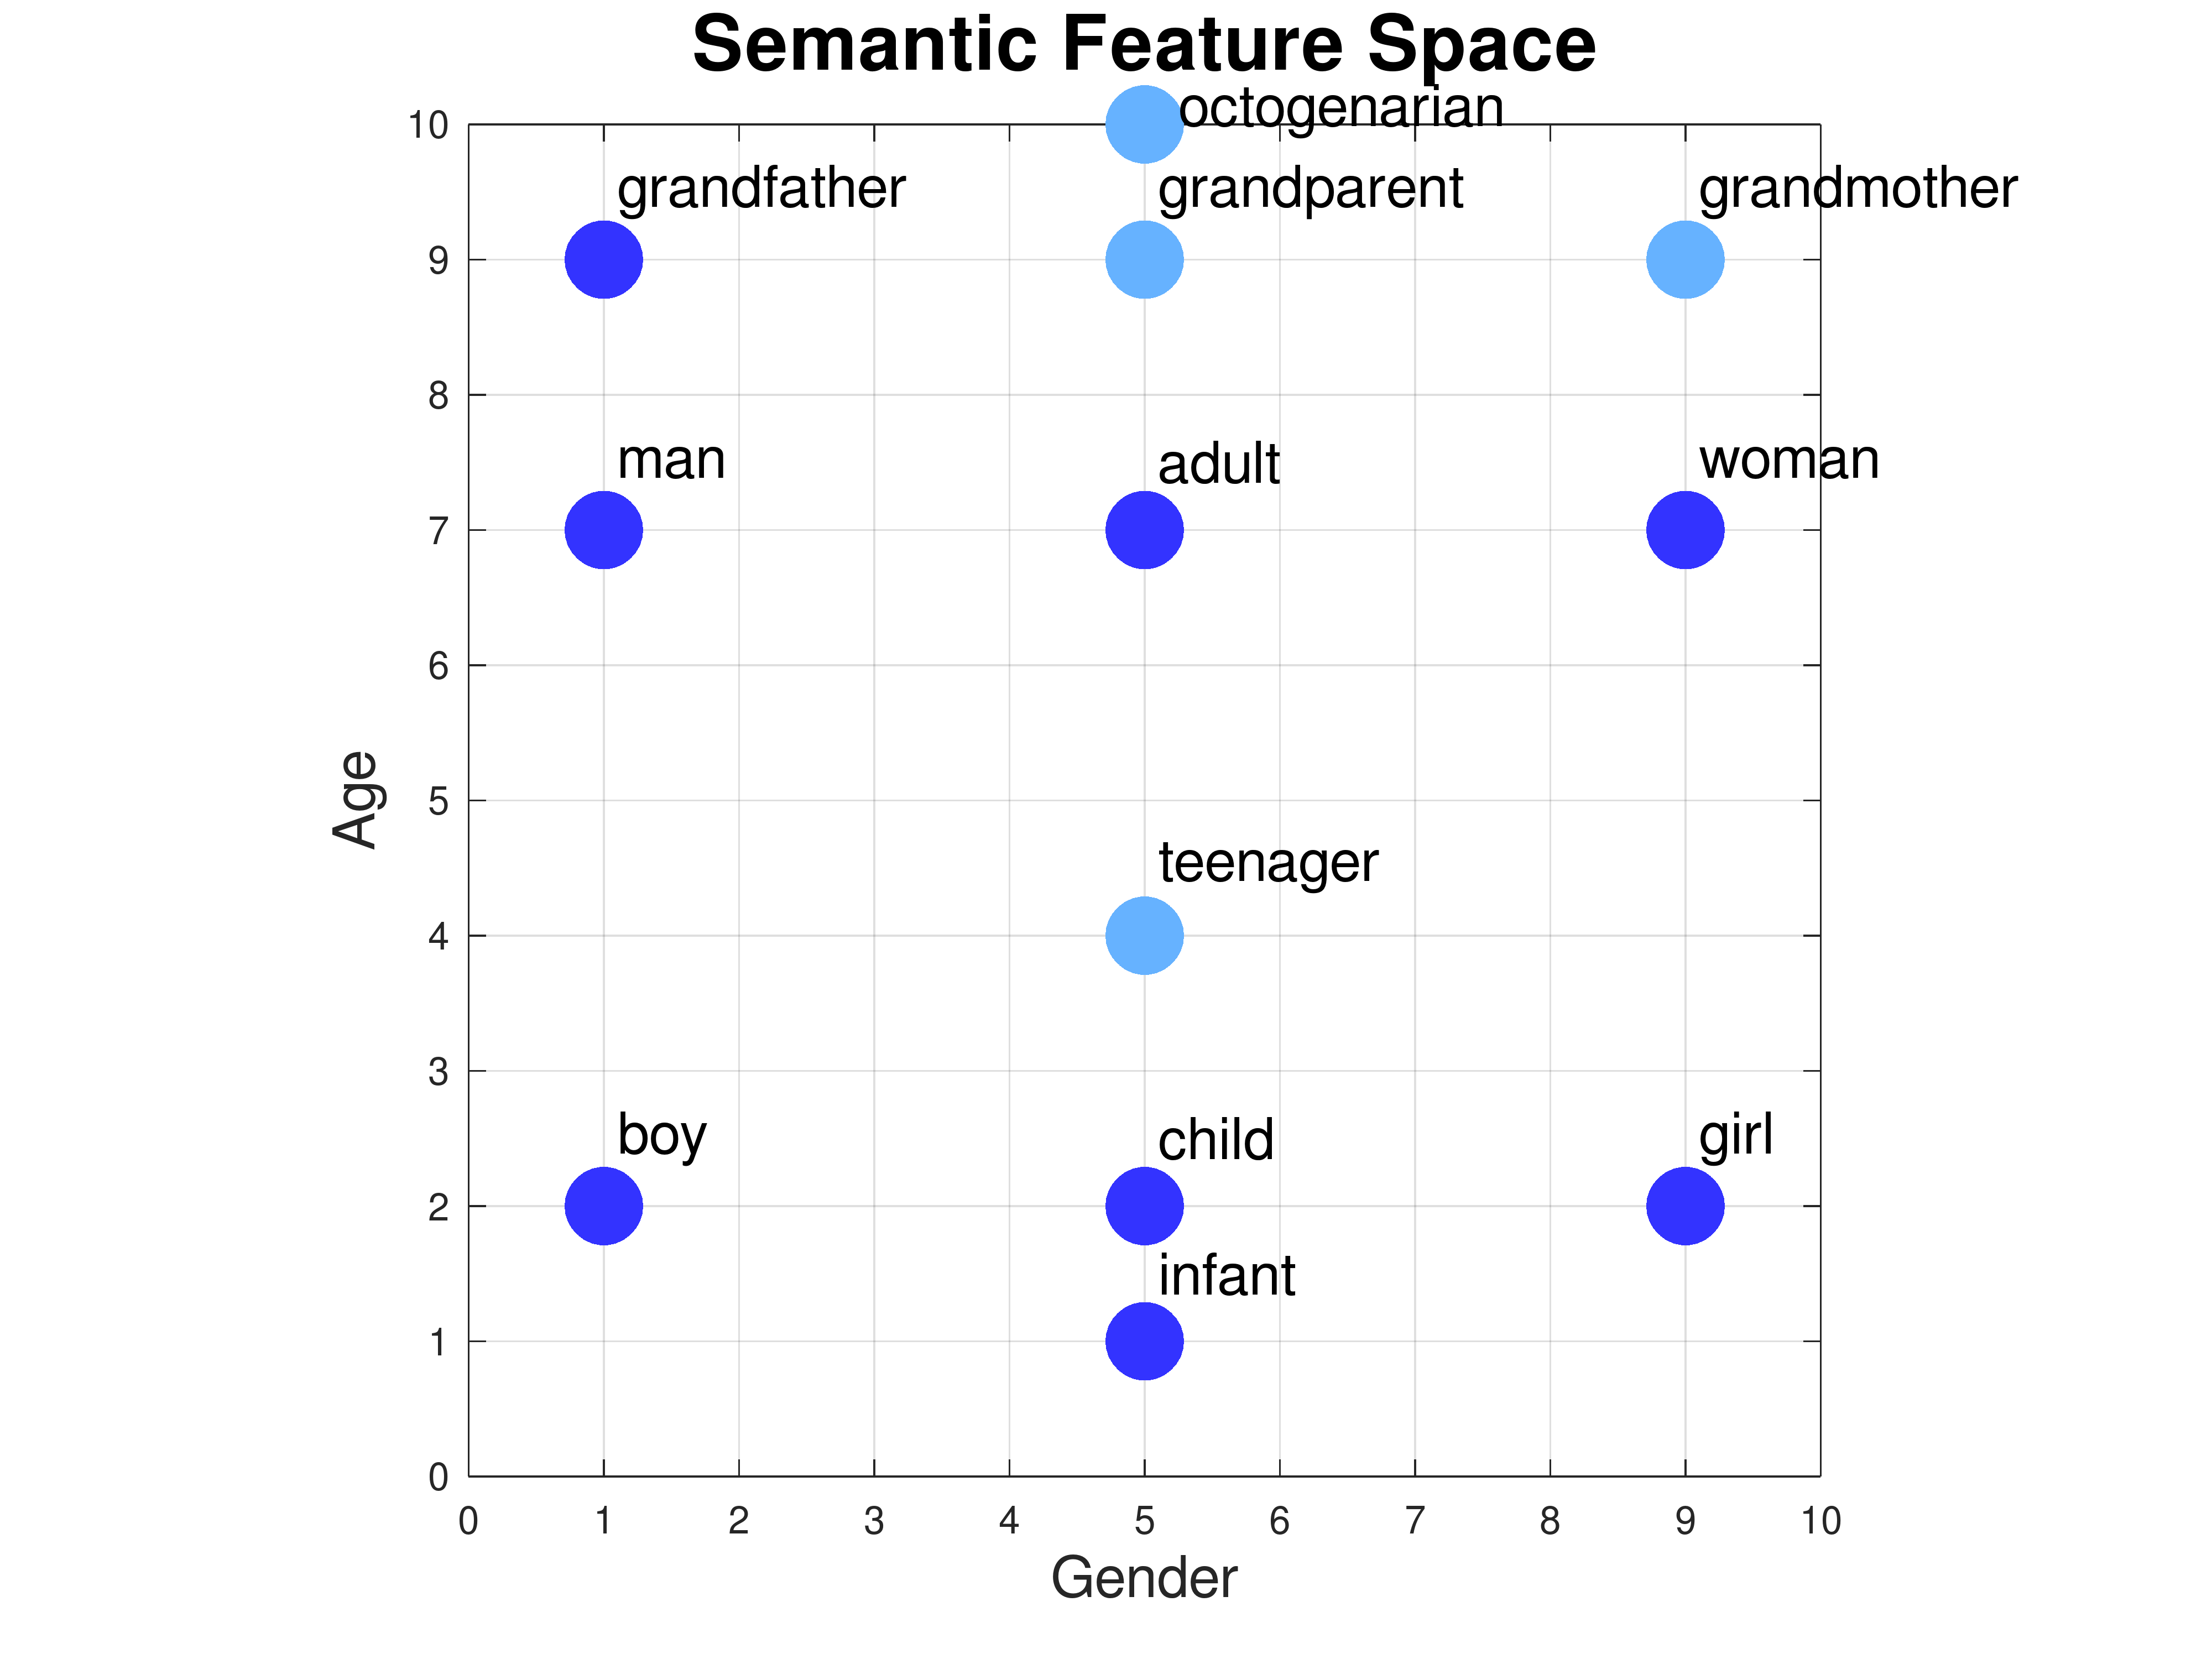
\includegraphics[width=\textwidth]{images/semantic_vectors.png}
      \end{figure}
    \end{column}
  \end{columns}
\end{frame}

\begin{frame}{Wortvektoren und Einbettungen (Embeddings)}
  \begin{columns}
    \begin{column}{1\textwidth}
      \begin{itemize}
        \item Ziel: Repräsentation von Wörtern in einem kontinuierlichen Vektorraum.
        \item Mathematische Definition:
          \begin{itemize}
            \item Gegeben eine Menge von Wörtern \( W = \{w_1, w_2, \dots, w_n\} \).
            \item Eine Einbettung ist eine Funktion \( f: W \to \mathbb{R}^d \), wobei \( d \) die Dimension des Vektorraums ist.
            \item Beispiel: \( f(w_i) = \mathbf{v}_i \in \mathbb{R}^d \).
          \end{itemize}
        \item Vorteile:
          \begin{itemize}
            \item Semantische Ähnlichkeit wird durch Nähe im Vektorraum dargestellt.
            \item Reduktion der Dimensionalität im Vergleich zu One-Hot-Encoding.
          \end{itemize}
      \end{itemize}
    \end{column}
    %\begin{column}{0.0\textwidth}
    %  \begin{figure}
    %    \centering
    %    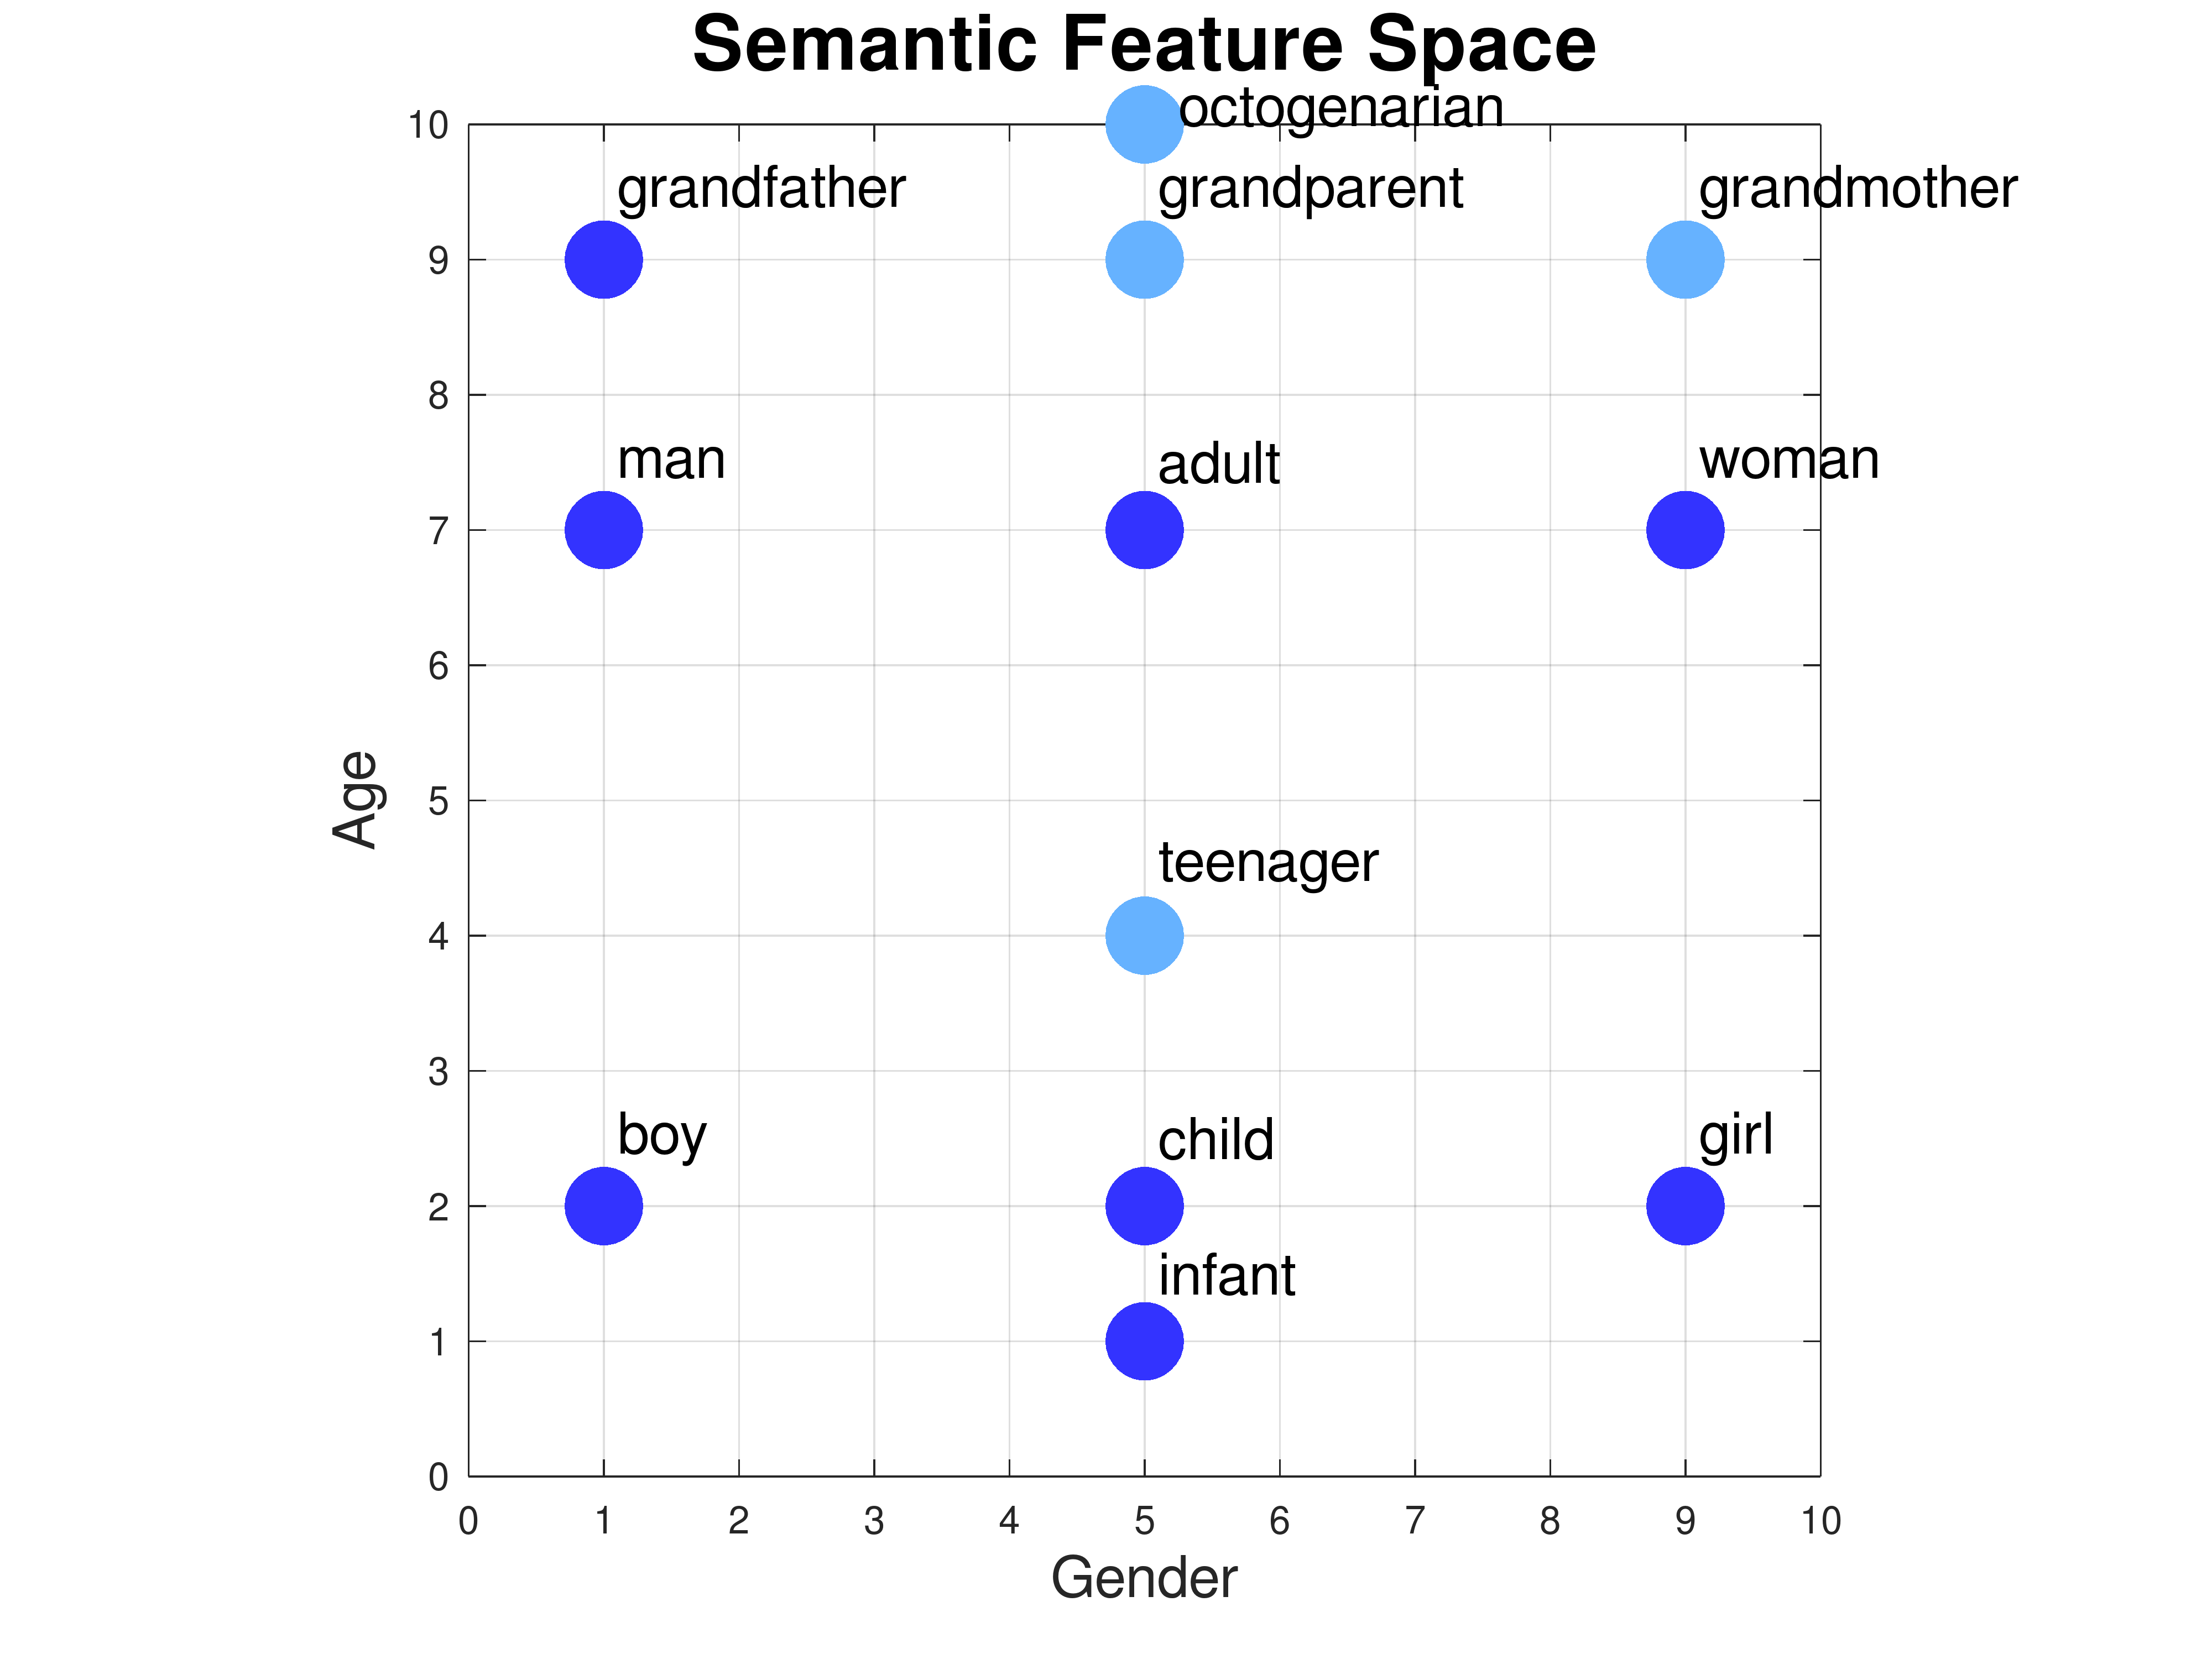
\includegraphics[width=\textwidth]{images/semantic_vectors.png}
    %  \end{figure}
    %\end{column}
  \end{columns}
\end{frame}

\begin{frame}{One-Hot-Encoding vs. Verteilte Repräsentationen}
  \begin{itemize}
    \item \textbf{One-Hot-Encoding:}
      \begin{itemize}
        \item Jedes Wort wird als Vektor mit einer einzigen Eins und sonst Nullen dargestellt.
        \item Beispiel: Für \( W = \{w_1, w_2, w_3\} \), \( w_2 \) wird als \( [0, 1, 0] \) kodiert.
        \item Nachteile: Hohe Dimensionalität, keine semantische Information.
      \end{itemize}
    \item \textbf{Verteilte Repräsentationen:}
      \begin{itemize}
        \item Nutzen kontinuierliche Vektorräume, um semantische Beziehungen darzustellen\footnote{Mikolov, T., Chen, K., Corrado, G., \& Dean, J. (2013). Efficient Estimation of Word Representations in Vector Space. arXiv preprint arXiv:1301.3781.}..
        \item Ermöglichen die Nutzung von Modellen wie Word2Vec und GloVe
        \footnote{Pennington, J., Socher, R., \& Manning, C. (2014). GloVe: Global Vectors for Word Representation. Proceedings of the 2014 Conference on Empirical Methods in Natural Language Processing (EMNLP).}.
        \item Wörter werden als dichte Vektoren in einem "niedrig"dimensionalen Raum dargestellt.
        \item Semantisch ähnliche Wörter haben ähnliche Vektoren.
        \item Beispiel: \( f(w_1) = [0.2, 0.8], f(w_2) = [0.3, 0.7] \).
      \end{itemize}
  \end{itemize}
\end{frame}

\begin{frame}{Word2Vec, GloVe und andere Einbettungsmethoden}
  \begin{itemize}
    \item \textbf{Word2Vec:}
      \begin{itemize}
        \item Skip-Gram-Modell: Vorhersage des Kontexts basierend auf einem Zielwort\footnote{Das Skip-Gram-Modell versucht, für ein gegebenes Zielwort die umgebenden Kontextwörter vorherzusagen.}.
        \item CBOW-Modell: Vorhersage des Zielworts basierend auf dem Kontext\footnote{Das Continuous Bag of Words (CBOW)-Modell sagt ein Zielwort basierend auf den umgebenden Kontextwörtern vorher. Es ist effizienter als das Skip-Gram-Modell, aber weniger präzise bei seltenen Wörtern.}.
      \end{itemize}
    \item \textbf{GloVe (Global Vectors for Word Representation):}
      \begin{itemize}
        \item Nutzt globale Wort-Kooccurenz-Matrizen\footnote{GloVe basiert auf der Idee, dass die globale Häufigkeit von Wortpaaren in einem Korpus genutzt werden kann, um semantische Beziehungen zwischen Wörtern zu modellieren.}.
        \item Optimiert eine Zielfunktion, die Wortpaare und ihre Häufigkeiten berücksichtigt\footnote{Die Zielfunktion von GloVe minimiert den Unterschied zwischen der inneren Produktdarstellung von Wortvektoren und der logarithmierten Häufigkeit von Wortpaaren.}.
      \end{itemize}
    \item \textbf{Andere Methoden:}
      \begin{itemize}
        \item FastText: Berücksichtigt Subwortinformationen.
        \item BERT-Embeddings: Kontextabhängige Einbettungen.
      \end{itemize}
  \end{itemize}
\end{frame}

\begin{frame}{Neuartige Embeddings (Teil 1)}
  \begin{itemize}
    \item \textbf{Kontextabhängige Embeddings:}
      \begin{itemize}
        \item Modelle wie BERT\footnote{Devlin, J., Chang, M.-W., Lee, K., \& Toutanova, K. (2019). BERT: Pre-training of Deep Bidirectional Transformers for Language Understanding. \url{https://arxiv.org/abs/1810.04805}}, GPT\footnote{Brown, T. et al. (2020). Language Models are Few-Shot Learners. \url{https://arxiv.org/abs/2005.14165}} und T5\footnote{Raffel, C. et al. (2020). Exploring the Limits of Transfer Learning with a Unified Text-to-Text Transformer. \url{https://arxiv.org/abs/1910.10683}} generieren Embeddings, die den Kontext eines Wortes berücksichtigen.
        \item Beispiel: Das Wort "Bank" hat unterschiedliche Embeddings in den Sätzen "Ich sitze auf der Bank" und "Ich gehe zur Bank".
      \end{itemize}
    \item \textbf{Sentence Embeddings:}
      \begin{itemize}
        \item Repräsentieren ganze Sätze statt einzelner Wörter.
        \item Modelle wie Sentence-BERT (SBERT)\footnote{Reimers, N., \& Gurevych, I. (2019). Sentence-BERT: Sentence Embeddings using Siamese BERT-Networks. \url{https://arxiv.org/abs/1908.10084}} ermöglichen semantische Suche und Textähnlichkeitsbewertung.
      \end{itemize}
  \end{itemize}
\end{frame}

\begin{frame}{Neuartige Embeddings (Teil 2)}
  \begin{itemize}
    \item \textbf{Multimodale Embeddings:}
      \begin{itemize}
        \item Kombinieren Informationen aus verschiedenen Modalitäten wie Text, Bild und Audio.
        \item Beispiel: CLIP (Contrastive Language–Image Pretraining)\footnote{Radford, A. et al. (2021). Learning Transferable Visual Models From Natural Language Supervision. \url{https://arxiv.org/abs/2103.00020}} von OpenAI.
      \end{itemize}
    \item \textbf{Graphbasierte Embeddings:}
     \begin{itemize}
        \item Repräsentieren Wörter als Knoten in einem Graphen, wobei Kanten Beziehungen zwischen Wörtern darstellen.
        \item Beispiel: Node2Vec\footnote{Grover, A., \& Leskovec, J. (2016). node2vec: Scalable Feature Learning for Networks. \url{https://arxiv.org/abs/1607.00653}} und GraphSAGE\footnote{Hamilton, W. et al. (2017). Inductive Representation Learning on Large Graphs. \url{https://arxiv.org/abs/1706.02216}}.
      \end{itemize}
    \item \textbf{Adapter-basierte Embeddings:}
      \begin{itemize}
        \item Ermöglichen die Anpassung vortrainierter Modelle an spezifische Aufgaben durch leichte Modifikationen.
        \item Reduzieren den Speicherbedarf im Vergleich zu vollständigem Fine-Tuning\footnote{Houlsby, N. et al. (2019). Parameter-Efficient Transfer Learning for NLP. \url{https://arxiv.org/abs/1902.00751}}.
      \end{itemize}
  \end{itemize}
\end{frame}

\begin{frame}{Text Preprocessing Pipeline}
  \begin{tikzpicture}[scale=0.8, transform shape]
    % Main arrow
    % Large arrow
    \fill[blue!50] (-1.5,-1.5) -- (10.5,-1.5) -- (10.5,-2) -- (17.5,0) -- (10.5,2) -- (10.5,1.5) -- (-1.5,1.5) -- cycle;

    % Process boxes
    \node (step1) [process, xshift=0cm] {Data Cleaning};
    \node (step2) [process, right of=step1, xshift=2.5cm] {Tokenization};
    \node (step3) [process, right of=step2, xshift=2.5cm] {Normalization};
    \node (step4) [process, right of=step3, xshift=2.5cm] {Stopword Removal};
    \node (step5) [process, right of=step4, xshift=2.5cm] {Vectorization};

    % Arrows connecting steps
    \draw[arrow] (step1.east) -- (step2.west);
    \draw[arrow] (step2.east) -- (step3.west);
    \draw[arrow] (step3.east) -- (step4.west);
    \draw[arrow] (step4.east) -- (step5.west);
  \end{tikzpicture}
\end{frame}

% Abschnitt 3: Attention-Mechanismus
\section{Attention-Mechanismus}

\begin{frame}{Attention-Mechanismus}
  \begin{itemize}
    \item Motivation für Attention in Sequenzmodellen
    \item Funktionsweise des Attention-Mechanismus
    \item Unterschied zwischen Self-Attention und Cross-Attention
  \end{itemize}
\end{frame}

\begin{frame}{Motivation für Attention in Sequenzmodellen}
  \begin{itemize}
    \item Problem: In langen Sequenzen verlieren Modelle wie RNNs und LSTMs den Überblick über frühere Informationen.
    \item Lösung: Der Attention-Mechanismus ermöglicht es, gezielt auf relevante Teile der Eingabesequenz zu fokussieren.
    \item Beispiel: Bei der Übersetzung eines Satzes kann Attention bestimmen, welches Wort im Quelltext für ein bestimmtes Wort im Zieltext wichtig ist.
  \end{itemize}
\end{frame}

\begin{frame}{Funktionsweise des Attention-Mechanismus}
  \begin{itemize}
    \item \textbf{Gegeben:} Eine Eingabesequenz mit \( n \) Elementen \( \{x_1, x_2, \dots, x_n\} \).
    \item \textbf{Ziel:} Berechnung einer gewichteten Summe der Eingaben, wobei die Gewichte die Relevanz jedes Elements darstellen.
    \item \textbf{Schritte:}
      \begin{enumerate}
        \item \textbf{Berechnung der Scores:}
        \[
        e_{ij} = \text{score}(h_i, h_j), \quad \text{wobei } h_i \text{ und } h_j \text{ die Hidden States sind.}
        \]
        \item \textbf{Normalisierung der Scores:}
        \[
        \alpha_{ij} = \frac{\exp(e_{ij})}{\sum_{k=1}^n \exp(e_{ik})} \quad \text{(Softmax)}.
        \]
        \item \textbf{Gewichtete Summe:}
        \[
        z_i = \sum_{j=1}^n \alpha_{ij} h_j.
        \]
      \end{enumerate}
  \end{itemize}
  \vspace{0.5cm}
  \begin{equation}
    \text{Attention}(Q, K, V) = \text{softmax}\left(\frac{QK^\top}{\sqrt{d_k}}\right)V
  \end{equation}
  Hierbei sind \( Q \) (Query), \( K \) (Key) und \( V \) (Value) Matrizen, und \( d_k \) ist die Dimension der Keys.
\end{frame}

\begin{frame}{Funktionsweise des Attention-Mechanismus}
  \centering
  \resizebox{0.6\textwidth}{0.9\textheight}{ % Resize to fit on slide
    \begin{tikzpicture}[
      every node/.style={draw, minimum width=0.5cm, minimum height=0.3cm, text centered, font=\tiny},
        arrow/.style={thick,->,>=stealth}
          ]
        % Input embeddings
        \node (input1) [rectangle, fill=blue!20] at (0,2) {Input 1};
        \node (input2) [rectangle, fill=blue!20, right=of input1, xshift=1.5cm] {Input 2};
        \node (input3) [rectangle, fill=blue!20, right=of input2, xshift=1.5cm] {Input 3};

        % Linear layers (Query, Key, Value)
        \node (query) [rectangle, fill=green!20, below=of input1, yshift=-0.1cm] {Query (Q)};
        \node (key) [rectangle, fill=yellow!20, below=of input2, yshift=-0.1cm] {Key (K)};
        \node (value) [rectangle, fill=red!20, below=of input3, yshift=-0.1cm] {Value (V)};

        % Attention Scores (QK^T / sqrt(d_k))
        \node (scores) [rectangle, fill=gray!20, below=of key, yshift=-0.2cm, minimum width=5cm] {$QK^T / \sqrt{d_k}$};

        % Softmax layer
        \node (softmax) [rectangle, fill=orange!30, below=of scores, yshift=-0.1cm, minimum width=3.5cm] {Softmax};

        % Weighted Sum of Values
        \node (weighted_sum) [rectangle, fill=red!30, below=of softmax, yshift=-0.1cm, minimum width=3cm] {Weighted Sum};

        % Output Embedding
        \node (output) [rectangle, fill=purple!30, below=of weighted_sum, yshift=-0.1cm] {Output};

        % Arrows with bends for compact layout
        \draw [arrow] (input1.south) -- (query.north);
        \draw [arrow] (input2.south) -- (key.north);
        \draw [arrow] (input3.south) -- (value.north);

        \draw [arrow] (query.south) |- (scores.west);
        \draw [arrow] (key.south) -- (scores.north);

        \draw [arrow] (scores.south) -- (softmax.north);
        \draw [arrow] (softmax.south) -- (weighted_sum.north);

        \draw [arrow] (value.south) |- (weighted_sum.east);
        \draw [arrow] (weighted_sum.south) -- (output.north);

          \end{tikzpicture}
}
\end{frame}

\begin{frame}{Self-Attention vs. Cross-Attention}
  \begin{columns}
    \begin{column}{0.5\textwidth}
      \textbf{Self-Attention:}
      \begin{itemize}
      \item Jeder Token in der Sequenz bezieht sich auf alle anderen Tokens in derselben Sequenz.
      \item Beispiel: Kontextualisierung eines Wortes in einem Satz.
      \end{itemize}
      \[
      \text{Attention}(Q, K, V) = \text{softmax}\left(\frac{QK^\top}{\sqrt{d_k}}\right)V, \quad Q = K = V
      \]
    \end{column}
    \begin{column}{0.5\textwidth}
      \textbf{Cross-Attention:}
      \begin{itemize}
      \item Tokens in einer Sequenz beziehen sich auf Tokens in einer anderen Sequenz.
      \item Beispiel: Übersetzung, bei der der Zieltext auf den Quelltext achtet.
      \end{itemize}
      \[
      \text{Attention}(Q, K, V) = \text{softmax}\left(\frac{QK^\top}{\sqrt{d_k}}\right)V, \quad Q \neq K = V
      \]
    \end{column}
    \end{columns}
\end{frame}
\begin{frame}{Self-Attention vs. Cross-Attention}
  \begin{columns}
    % Self-Attention Diagram
    \begin{column}{0.5\textwidth}
      \centering
      \resizebox{0.9\textwidth}{!}{ % Resize to fit within column
      \begin{tikzpicture}[
        every node/.style={draw, minimum width=0.7cm, minimum height=0.5cm, text centered, font=\scriptsize},
        arrow/.style={thick,->,>=stealth}
      ]
        % Self-Attention Section
        \node (self_input1) [rectangle, fill=blue!20] at (0,4) {Input 1};
        \node (self_input2) [rectangle, fill=blue!20, right=of self_input1, xshift=1.5cm] {Input 2};
        \node (self_input3) [rectangle, fill=blue!20, right=of self_input2, xshift=1.5cm] {Input 3};

        \node (self_q) [rectangle, fill=green!20, below=of self_input1, yshift=-0.25cm] {Query (Q)};
        \node (self_k) [rectangle, fill=yellow!20, below=of self_input2, yshift=-0.25cm] {Key (K)};
        \node (self_v) [rectangle, fill=red!20, below=of self_input3, yshift=-0.25cm] {Value (V)};

        \node (self_attention) [rectangle, fill=gray!20, below=of self_k, yshift=-0.25cm, minimum width=5cm] {$QK^T / \sqrt{d_k}$};
        \node (self_output) [rectangle, fill=purple!30, below=of self_attention, yshift=-0.25cm] {Self-Attention Output};

        % Arrows for Self-Attention
        \draw [arrow] (self_input1.south) -- (self_q.north);
        \draw [arrow] (self_input2.south) -- (self_k.north);
        \draw [arrow] (self_input3.south) -- (self_v.north);
        \draw [arrow] (self_q.south) |- (self_attention.west);
        \draw [arrow] (self_k.south) -- (self_attention.north);
        \draw [arrow] (self_v.south) |- (self_attention.east);
        \draw [arrow] (self_attention.south) -- (self_output.north);

        % Labels
        \node at (3.25, 4.5) {\textbf{Self-Attention (Same Input)}};
      \end{tikzpicture}
      }
    \end{column}

    % Cross-Attention Diagram
    \begin{column}{0.5\textwidth}
      \centering
      \resizebox{0.9\textwidth}{!}{ % Resize to fit within column
      \begin{tikzpicture}[
        every node/.style={draw, minimum width=0.7cm, minimum height=0.5cm, text centered, font=\scriptsize},
        arrow/.style={thick,->,>=stealth}
      ]
        % Cross-Attention Section
        \node (cross_q) [rectangle, fill=green!20] at (0,4) {Query (Q) (Decoder)};
        \node (cross_k) [rectangle, fill=yellow!20, right=of cross_q, xshift=3cm] {Key (K) (Encoder)};
        \node (cross_v) [rectangle, fill=red!20, right=of cross_k, xshift=2cm] {Value (V) (Encoder)};

        \node (cross_attention) [rectangle, fill=gray!20, below=of cross_k, yshift=-0.25cm, minimum width=5cm] {$QK^T / \sqrt{d_k}$};
        \node (cross_output) [rectangle, fill=purple!30, below=of cross_attention, yshift=-0.25cm] {Cross-Attention Output};

        % Arrows for Cross-Attention
        \draw [arrow] (cross_q.south) |- (cross_attention.west);
        \draw [arrow] (cross_k.south) -- (cross_attention.north);
        \draw [arrow] (cross_v.south) |- (cross_attention.east);
        \draw [arrow] (cross_attention.south) -- (cross_output.north);

        % Labels
        \node at (5.5, 4.5) {\textbf{Cross-Attention (Decoder-Encoder)}};
      \end{tikzpicture}
      }
    \end{column}
  \end{columns}
\end{frame}

\begin{frame}{Visualisierung der Attention-Matrix}
  \begin{itemize}
    \item Die Attention-Matrix zeigt die Gewichte \( \alpha_{ij} \), die die Relevanz von Token \( j \) für Token \( i \) darstellen.
    \item Beispiel: Bei der Übersetzung eines Satzes zeigt die Matrix, welche Wörter im Quelltext für ein bestimmtes Wort im Zieltext wichtig sind.
  \end{itemize}
  \begin{figure}
    \centering
    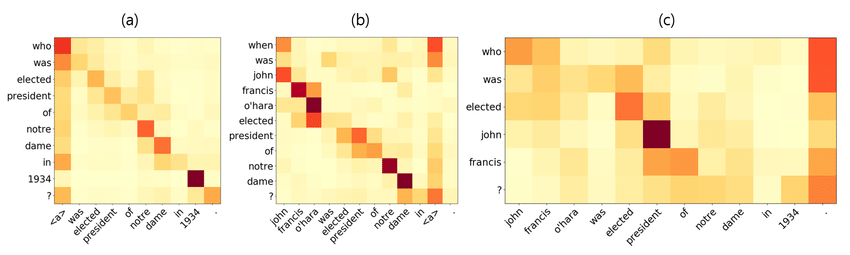
\includegraphics[width=0.8\textwidth]{images/attention_matrix.png}
    \caption{Beispiel einer Attention-Matrix. Kim, Yanghoon \& Hwanhee, Lee \& Shin, Joongbo \& Jung, Kyomin. (2018). Improving Neural Question Generation using Answer Separation. 10.48550/arXiv.1809.02393. }
  \end{figure}
\end{frame}

% Abschnitt 4: Transformer-Architektur
\section{Transformer-Architektur}

\begin{frame}{Transformer-Architektur}
  \begin{itemize}
    \item Überblick über die Transformer-Architektur
    \item Encoder-Decoder-Struktur
    \item Vorteile gegenüber rekurrenten Netzwerken
  \end{itemize}
\end{frame}

% Abschnitt 5: Von BERT zu DeepSeek-v3
\section{Von BERT zu DeepSeek-v3}

\begin{frame}{Von BERT zu DeepSeek-v3}
  \begin{itemize}
    \item Einführung in BERT und seine Architektur
    \item Weiterentwicklungen: GPT, RoBERTa, T5
    \item Überblick über DeepSeek-v3 und seine Besonderheiten
  \end{itemize}
\end{frame}

% Abschnitt 6: Zukunftsperspektiven
\section{Wie es weitergehen kann}

\begin{frame}{Wie es weitergehen kann}
  \begin{itemize}
    \item Aktuelle Forschungstrends im NLP
    \item Herausforderungen und offene Fragen
    \item Ethische Überlegungen und gesellschaftliche Auswirkungen
  \end{itemize}
\end{frame}

% Abschnitt 7: Nutzungsmöglichkeiten: RAG, Agentensysteme
\section{Nutzungsmöglichkeiten: RAG, Agentensysteme}

\begin{frame}{Nutzungsmöglichkeiten: RAG, Agentensysteme}
  \begin{itemize}
    \item Retrieval-Augmented Generation (RAG) und seine Anwendungen
    \item Entwicklung und Einsatz von Agentensystemen im NLP
    \item Kombination von LLMs mit externem Wissen
  \end{itemize}
\end{frame}


% Abschnitt 8: AI Safety und Ethik
\section{AI Safety und Ethik}
\begin{frame}{AI Safety und Ethik}
  \begin{columns}
    \begin{column}{1\textwidth}
      \begin{itemize}
        \item Bedeutung von Sicherheit und Ethik in der KI-Entwicklung
        \item Risiken und Herausforderungen bei der Nutzung von LLMs
        \item Ansätze zur Förderung von verantwortungsvoller KI
      \end{itemize}
    \end{column}
    %\begin{column}{0.3\textwidth}
    %  \begin{figure}
    %    \centering
    %    \includegraphics[width=\textwidth]{images/ai_safety.png}
    %  \end{figure}
    %\end{column}
  \end{columns}
\end{frame}

\begin{frame}{Bedeutung von Sicherheit und Ethik}
  \begin{columns}
    \begin{column}{1\textwidth}
      \begin{itemize}
        \item \textbf{Sicherheit:} Verhindern von Fehlverhalten oder schädlichem Verhalten durch KI-Systeme.
        \item \textbf{Ethik:} Sicherstellen, dass KI-Systeme fair, transparent und respektvoll gegenüber menschlichen Werten sind.
        \item \textbf{Gesellschaftliche Auswirkungen:} Einfluss von KI auf Arbeitsplätze, Privatsphäre und soziale Gerechtigkeit.
      \end{itemize}
    \end{column}
    %\begin{column}{0.3\textwidth}
    %  \begin{figure}
    %    \centering
    %    \includegraphics[width=\textwidth]{images/ethics.png}
    %  \end{figure}
    %\end{column}
  \end{columns}
\end{frame}

\begin{frame}{Risiken und Herausforderungen}
  \begin{columns}
    \begin{column}{1\textwidth}
      \begin{itemize}
        \item \textbf{Bias und Diskriminierung:} LLMs können Vorurteile aus Trainingsdaten übernehmen.
        \item \textbf{Desinformation:} Generierung von falschen oder irreführenden Inhalten.
        \item \textbf{Missbrauch:} Einsatz von LLMs für schädliche Zwecke wie Phishing oder Propaganda.
        \item \textbf{Black-Box-Problem:} Mangel an Transparenz und Nachvollziehbarkeit in KI-Modellen.
      \end{itemize}
    \end{column}
    %\begin{column}{0.3\textwidth}
    %  \begin{figure}
    %    \centering
    %    \includegraphics[width=\textwidth]{images/challenges.png}
    %  \end{figure}
    %\end{column}
  \end{columns}
\end{frame}

\begin{frame}{Ansätze zur Förderung von verantwortungsvoller KI}
  \begin{columns}
    \begin{column}{1\textwidth}
      \begin{itemize}
        \item \textbf{Regulierung und Richtlinien:} Entwicklung von Standards und Gesetzen für den Einsatz von KI.
        \item \textbf{Technische Lösungen:} 
          \begin{itemize}
            \item Bias-Detektion und -Korrektur.
            \item Explainable AI (XAI) zur Verbesserung der Transparenz. 
          \end{itemize}
        \item \textbf{Bildung und Bewusstsein:} Förderung von Wissen über KI-Sicherheit und Ethik in der Gesellschaft.
        \item \textbf{Zusammenarbeit:} Interdisziplinäre Ansätze zwischen Technik, Recht und Philosophie.
      \end{itemize}
    \end{column}
    %\begin{column}{0.3\textwidth}
    %  \begin{figure}
    %    \centering
    %    \includegraphics[width=\textwidth]{images/responsible_ai.png}
    %  \end{figure}
    %\end{column}
  \end{columns}
\end{frame}


\begin{frame}{LLM Standardwerke}
\begin{itemize}
\item \textbf{Build LLMs from Scratch} (Raschka)
\begin{itemize}
\item \url{https://github.com/rasbt/LLMs-from-scratch}
\item Praktische Implementierung in PyTorch
\end{itemize}

\item \textbf{Transformers for NLP} (Rothman)
\begin{itemize}
\item ISBN 978-1803247335
\item BERT/GPT Anwendungen
\end{itemize}
\end{itemize}
\end{frame}

\begin{frame}{LLM Forschungsarbeiten}
\begin{itemize}
\item \textbf{Attention Is All You Need} (2017)
\begin{itemize}
\item \url{https://arxiv.org/abs/1706.03762}
\item Transformer-Architektur
\end{itemize}

\item \textbf{BERT Paper} (Devlin 2019)
\begin{itemize}
\item \url{https://arxiv.org/abs/1810.04805}
\item Bidirektionale Pretraining
\end{itemize}

\item \textbf{GPT-3 Paper} (Brown 2020)
\begin{itemize}
\item \url{https://arxiv.org/abs/2005.14165}
\item Few-Shot Learning
\end{itemize}
\end{itemize}
\end{frame}

\begin{frame}{LLM Praktische Ressourcen}
\begin{itemize}
\item \textbf{Hugging Face Transformers}
\begin{itemize}
\item \url{https://github.com/huggingface/transformers}
\end{itemize}

\item \textbf{LangChain}
\begin{itemize}
\item \url{https://python.langchain.com/}
\item LLM Orchestrierung
\end{itemize}

\item \textbf{LLaMA \& LlamaIndex}
\begin{itemize}
\item \url{https://github.com/facebookresearch/llama}
\item Open-Weight Modelle
\end{itemize}
\end{itemize}
\end{frame}
\begin{frame}[allowframebreaks]{References}
 \bibliographystyle{ieeetr}
 \bibliography{lit.bib}
\end{frame}
\end{document}
